%----------------------------------------------------------------------------------------
%PACKAGES AND OTHER DOCUMENT CONFIGURATIONS
%----------------------------------------------------------------------------------------

\documentclass[11pt]{article} 

\usepackage[top=.4in, bottom=1in, left=1in,
right=.3in]{geometry} 

\geometry{a4paper} 

\usepackage{graphicx}

\usepackage{float} 

\usepackage{wrapfig}

\linespread{1} % Line spacing

\usepackage{ragged2e}

\usepackage{enumitem}


%\setlength\parindent{0pt} % Uncomment to remove all indentation from
%paragraphs
\graphicspath{{../../pics/}} 


\begin{document}

\begin{center} \huge{\bfseries{Hierarchical goal abstraction for sensorimotor
    agency}}\\ {The model -- Draft 0.1 \today}\\[3cm] \end{center}


\begin{figure}[H] \centering \includegraphics[width=.8\textwidth]{schema}
    \caption{Architecture of the model.} \label{fig:blueprint} \end{figure}

\section{Simulator}

\begin{itemize}

    \item \textbf{Environment:} the simulation is done in a 2-dimensional space
        without physics.

    \item \textbf{Agent:} \begin{itemize}

            \item The whole body is composed of the 2 arms plus a segment
                joining their origins

            \item Each arm has 3 joints (3DoF)

            \item 22 touch sensors all over the body.

        \end{itemize}

    \item \textbf{Agent sensory information:}

        \begin{itemize}

            \item \texttt{vision (V):} a 20x20pixels retina on which the body
                (black line on figure~\ref{fig:blueprint}) is depicted in the
                current position.

            \item \texttt{proprioception (P):} a 20x20pixels retina on which
                the current angles of joints are represented.

                Encoding:

                \begin{itemize} 

                    \item Angles are encoded as 2D gaussians on a horizontal
                        line centered in the middle of the retina. 

                    \item The position of each gaussian on the horizontal line
                        is related to the position of the related joint in the
                        one-dimentional space of the body.

                    \item The variance of each gaussian on the y-axis is
                        related to the amplitude of the represented joint
                        angle.

                    \item The variance of each gaussian on the x-axis is a
                        proportion of the one on the y-axis, so that
                        overlapping between gaussians is not too much.

                \end{itemize} 

            \item \texttt{touch (T):} a 20x20pixels retina on which the current
                activations of the touch sensors are represented.

                Encoding:

                \begin{itemize} 

                    \item Sensors are encoded as 2D gaussians on a horizontal
                        line centered in the middle of the retina. 

                    \item The position of each gaussian on the horizontal line
                        is related to the position of the sensor in the
                        one-dimentional space of the body.

                    \item The variance of each gaussian on the y-axis is
                        related to the amplitude of the activation of the
                        represented sensor.

                    \item The variance of each gaussian on the x-axis is a
                        proportion of the one on the y-axis, so that gaussians
                        do not overlap too much.

                \end{itemize} 

        \end{itemize}

\end{itemize}



\section{Controller} The controller takes the sensory information at each
timestep and outputs a motor command consisting in the current requested
position of the 6 joint angles.

\subsection{Definitions}

\begin{itemize}[leftmargin=3cm]  
    \item[\textbf{goal:}]

        \begin{itemize}

            \item A state of the world that the \textbf{goal-abstraction layer}
                can identify and distinguish from others
                (section~\ref{sec:abstraction}).

            \item A configuration of the \textbf{action-selection layer} that
                can be linked to a proper action (section~\ref{sec:selection}).

        \end{itemize}

\end{itemize}

\begin{quote}
    Note: the goal-abstraction layer has the same dimensionality of\\ 
    \texttt{
        Note: the goal-abstraction layer has the same dimensionality of\\ 
        the goal-selection layer so that they can be compared.
    }

\end{quote}

\begin{itemize}[leftmargin=3cm]  

    \item[\textbf{match:}]

        \begin{itemize}

            \item The occurrence of an identical configuration of the
                goal-abstraction and goal-selection layers. 

        \end{itemize}    

    \item[\textbf{prediction:}]

        \begin{itemize}

            \item Computation of the probability that given a configuration of
                the goal-selection layer the agent will obtain a state in which
                the goal-abstraction layer has the same configuration
                (\emph{match} event). 

        \end{itemize}  

    \item[\textbf{error:}]

        \begin{itemize}

            \item Difference between the prediction and the real occurrence of
                a \emph{match} event within a trial.

        \end{itemize}  

\end{itemize} 

\label{sec:abstraction}

The sensory information is further processed by computing the finite difference
with the information given at the previous timestep. As a result the actual
input is composed by three retinas containing the \emph{derivatives} of the
(V), (P) and (T) retinas described above. 

The result of this processing is sent as input to a 4-layered hierarchical set
of self-organizing maps (SOMs). The output of each SOM is further processed so
that all output units have 0 activation except the one whose weights are the
closest to the current input, which has 1 activation.  There is a further
threshold based on the current learning within the SOM, so that if the weights
for the cluster to which the current input should belong have not been learned
enough then all output units have 0 activation.

In the 1st layer of the hierarchical network the segregation between sensory
modalities is maintained. Thus this layer is composed of three SOMs each
reducing the 20x20pixel input of a sensory modality to a 8x8pixel output.
%
\begin{figure}[H]
    \centering
    A 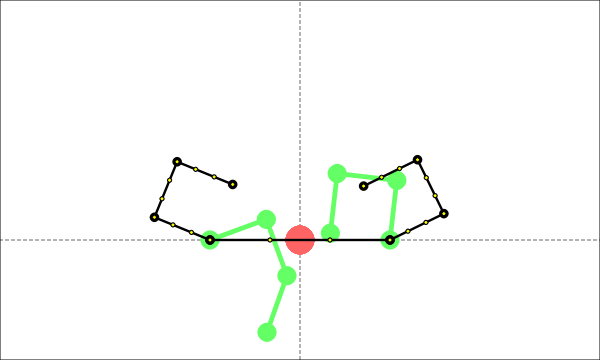
\includegraphics[width=.6\textwidth]{SOMs_kinematics}\\
    B 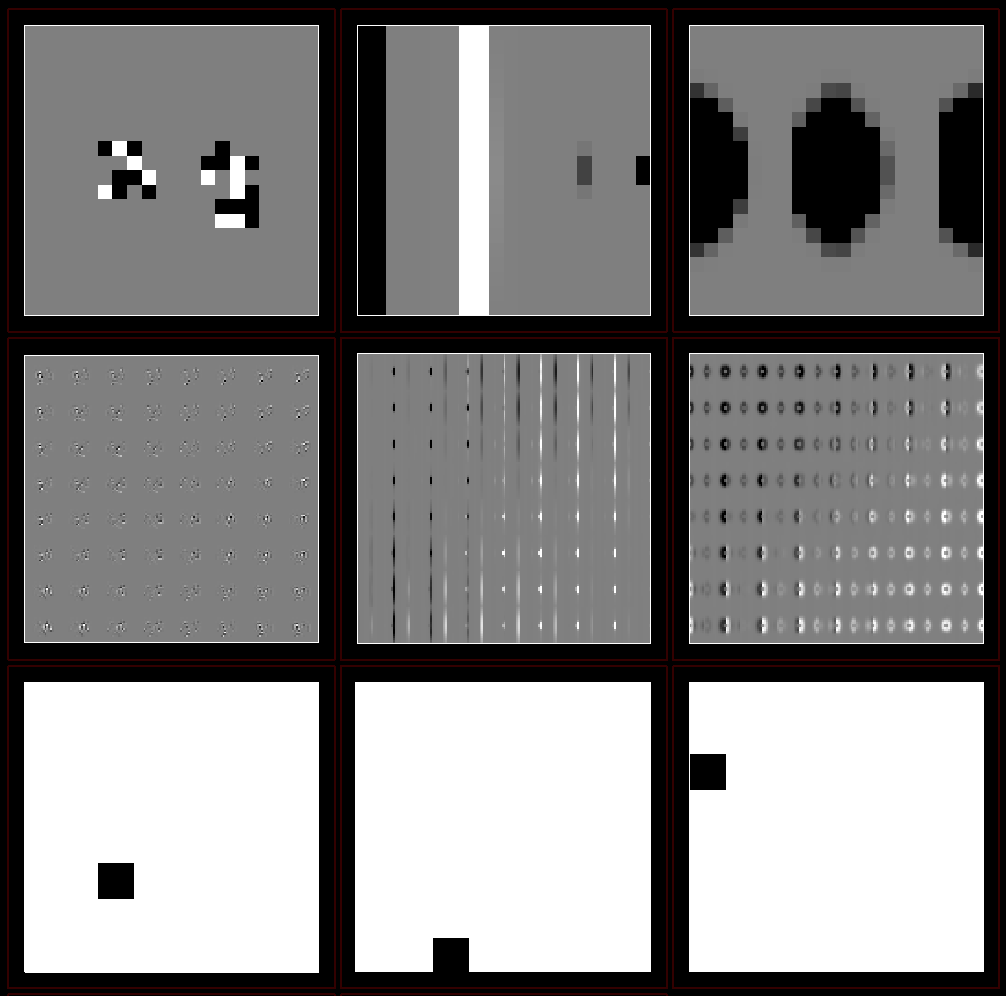
\includegraphics[width=.6\textwidth]{SOMs}

    \caption{
        Activity of the 1st layer of the hierarchical network. A) The
        current position of the agent. B) The first row shows the derivatives of
        the (V),(P) and (T) retinas. The second row show the current status of the 
        weights of the SOMs. Each of the three plots shows a 8x8 matrix of 
        20x20 retinas. Each 20x20 retina represents the weights connecting 
        the input retina to an output unit. The third row shows the output layers
        of each SOM. the black pixel represents the winner unit for the current input.
    }

    \label{fig:soms}
\end{figure}
%
The 2nd layer of the hierarchical network is composed of two SOMs. The 1st SOM in
the 2nd layer merges the 16x8pixel output coming from the (V) and the (P) SOMs
in the first layer into a 4x4pixel output. The 2st SOM in the 2nd layer merges
the 16x8pixel output coming from the (P) and the (T) SOMs in the first layer
into a further 4x4pixel output. The 3rd layer is composed by a single SOM
mergng the outputs of the 2nd layers (a 8x4pixels retina) into a 4x4pixels
output. The 4rd layer gets all the outputs from the previous layers as a
(3*400+2*32+16)pixels flatten input vector and merges it into a 3x3pixels
output. \textbf{The 4th layer gives abstracted representations of the 3-modal
    sensory information as 9 identifiable states.  }

\subsection{Goal selection}

\label{sec:selection}

The goal-selection layer is composed by a matrix of 3x3 units (same numerosity
of the goal-abstraction layer). At the start of each trial one of the units is
activated. The choice about which unit has to be activated is stochastic.  The
probability for each unit is given by applying a softmax to the amplitudes of
3x3 running averages of the prediction error (see
section~\ref{sec:prediction}). Each average is updated at the end of trials in
which the corresponding goal-selection unit is chosen. As a result these
running averages convey information about the current amount of error related
to each goal-selection unit. \textbf{Thus the probability of a goal to be
    selected is related to the amount of prediction error on it (intrinsic
motivation to learn what has not yet been learned).}

\subsection{Goal prediction}

\label{sec:prediction}

The \textbf{goal-prediction layer} takes the activation of the goal-selection
layer as an input and  outputs a \textbf{prediction of a \emph{match} event}
This prediction is compared with the actual occurrence of a \emph{match} event
at the end of each trial.  The result of this comparison (\emph{error}) is used
both to update the parameters of the goal-prediction layer and to decide the
activation of the goal-selection layer (see section \ref{sec:selection}).


\subsection{Action triggering}

The \textbf{motor output} of the controller is represented by the
activation of 6 readout units of an echo-state network (ESN). Each readout
units gives the current amplitude of a joint angle of the 2-arm agent. 
%
\begin{figure}[H]
    \centering
    A 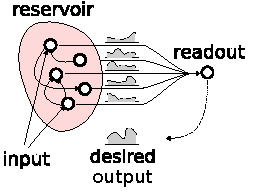
\includegraphics[width=.3\textwidth]{reservoir}
    B 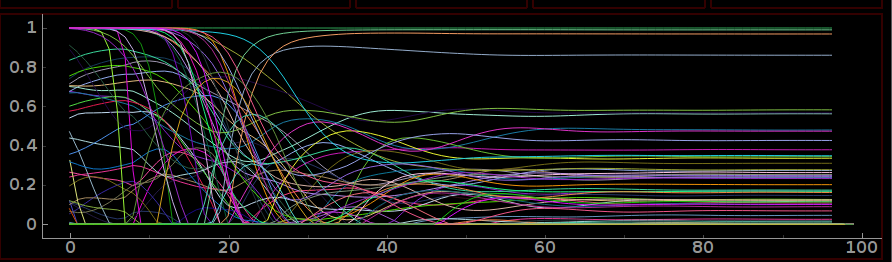
\includegraphics[width=.6\textwidth]{ESN}
    \caption{
        The echo-state network. A) General schema of the functioning of an ESN.
        Inputs reach sparsely the internal units of the reservoir.  Internal
        units are connected with each other via sparse random connections.
        Learning consists in the update of the external weights connecting the
        reservoir to one or more readout units. After learning the readout units
        reproduce a learned trajectory in relation to a specific input.
        B) The typical activation of the reservoir in the model. During the second 
        half of the trial the ESN reaches a fixed point that is peculiar of for 
        the current input (a selected goal).
    }
    \label{fig:esn}
\end{figure}
%
The input to the ESN is given by the goal-selection layer. The activation of
the goal-selection layer is connected to the ESN in two ways: 

\begin{enumerate}

    \item It steadily excitates distinct subpopulations of the ESN
        reservoir based on the current selection during a trial. This
        excitation triggers the proper dynamics of the reservoir and
        guaranties that the reservoir activity fades to a distinct fixed
        point depending on the selection.

    \item It inhibits distinct subpopulations of the ESN reservoir based on
        the current selection. This inhibition allows to select different
        dynamics in the network.

\end{enumerate}

The weights connecting the reservoir to the readout units of the ESN are
updated via a reward-based online learning rule. \textbf{The \emph{match}
event triggers the reward signal.} \\

The actual motor output is composed of the activation of the 6 readout units
and that of 6 sinusoidal oscillators whose parameters are set randomly at each
trial.  These oscillators add \textbf{exploratory} noise to the motor output.
Their amplitude depends on the amount of previous \emph{match} events given the
same selection.  As soon as matches become frequent the motor output becomes
completelly dependent on the activity of the readout units
(\textbf{exploitation}). 


\section{Simulation flow}

Each trial is composed of two phases:

\begin{itemize}

    \item \textbf{reset interval} no goal is selected, no update is made to the
        weights of the motor readout units and no goal input is given to the
        ESN. 

    \item \textbf{activation} all components are switched on. A goal is chosen
        in the goal-selection layer and is maintained fixed throughout the
        trial.

\end{itemize}

A trial ends if a determined amount of time is reached or if a match event
occurs.  At the end of each trial the prediction error is computed. The moving
average of the prediction error for the current selection is updated.


\end{document}



